% !TEX program = xelatex
\documentclass[UTF8,fontset=fandol,a4paper,11pt]{ctexart}
\usepackage[margin=21mm,top=23mm,bottom=22mm,headheight=16pt]{geometry}
\usepackage{amsmath,amssymb,mathtools,bm}
\usepackage{tikz}
\usetikzlibrary{arrows.meta,calc,angles,quotes,patterns}
\usepackage{xcolor,booktabs,array,longtable,enumitem,fancyhdr,needspace}
\usepackage[unicode,hidelinks]{hyperref}
\definecolor{ink}{HTML}{24343C}
\definecolor{accent}{HTML}{166A70}
\definecolor{muted}{HTML}{65747A}
\definecolor{rulegray}{HTML}{D4DDE0}
\definecolor{warm}{HTML}{966037}
\color{ink}
\setlength{\parindent}{2em}
\setlength{\parskip}{4pt}
\linespread{1.12}
\AtBeginDocument{\setlength{\abovedisplayskip}{6pt plus 2pt minus 1pt}
\setlength{\belowdisplayskip}{6pt plus 2pt minus 1pt}
\setlength{\abovedisplayshortskip}{0pt plus 1pt}
\setlength{\belowdisplayshortskip}{4pt plus 1pt}}
\setlist[enumerate]{label=(\arabic*),leftmargin=2.3em,itemsep=3pt,topsep=4pt}
\setlist[itemize]{leftmargin=2em,itemsep=2pt,topsep=4pt}
\allowdisplaybreaks[1]
\setlength{\emergencystretch}{2em}
\setcounter{secnumdepth}{0}
\providecommand{\tightlist}{\setlength{\itemsep}{0pt}\setlength{\parskip}{0pt}}
\ctexset{section={format=\Large\bfseries\color{accent},beforeskip=10pt,afterskip=9pt},
subsection={format=\normalsize\bfseries\color{accent},beforeskip=10pt,afterskip=4pt},
subsubsection={format=\normalsize\bfseries,beforeskip=8pt,afterskip=3pt}}
\pagestyle{fancy}
\fancyhf{}
\fancyhead[L]{\small\color{muted}物理学难题集萃}
% 页眉仅保留书名；版本名称只在封面显示。
\fancyfoot[L]{\small\color{muted}\chapterlabel}
\fancyfoot[R]{\small\thepage}
\renewcommand{\headrulewidth}{0.4pt}
\renewcommand{\footrulewidth}{0pt}
\newcommand{\dd}{\mathop{}\!\mathrm{d}}
\newcommand{\vect}[1]{\bm{#1}}
\newcommand{\tagline}[1]{\noindent{\small\color{muted}#1}\par}
\newcommand{\result}[1]{\begin{equation*}\boxed{#1}\end{equation*}}
\newcommand{\figcaption}[1]{\par\vspace{2pt}{\small\color{muted}#1}\par}
\newcommand{\teach}[2]{\Needspace{4\baselineskip}\subsection*{讲解要点与追问}#1\par\smallskip\noindent\textbf{追问：}#2\par}
\newcommand{\workarea}{\par\vspace{7mm}\noindent{\small\color{muted}作答区}\par\vspace{4mm}
\noindent\textcolor{rulegray}{\rule{\linewidth}{0.3pt}}\par\vspace{16mm}
\noindent\textcolor{rulegray}{\rule{\linewidth}{0.3pt}}\par\vspace{16mm}
\noindent\textcolor{rulegray}{\rule{\linewidth}{0.3pt}}\par\vspace{16mm}
\noindent\textcolor{rulegray}{\rule{\linewidth}{0.3pt}}}
\tikzset{axis/.style={-{Stealth[length=2mm]},thin,color=muted},
motion/.style={-{Stealth[length=2.3mm]},thick,color=accent},
force/.style={-{Stealth[length=2.3mm]},thick,color=warm},
traj/.style={thick,color=accent},guide/.style={dashed,thin,color=muted},
object/.style={thick,color=ink},every node/.style={font=\small}}\widowpenalty=10000\clubpenalty=10000\displaywidowpenalty=10000\newcommand{\chapterlabel}{电磁学试题（三）}







\hypersetup{pdftitle={电磁学试题（三）·学生版},pdfauthor={}}

\begin{document}\pdfbookmark[0]{电磁学试题（三）}{cover}

\thispagestyle{empty}\vspace*{22mm}

\noindent{\Huge\bfseries 物理学难题集萃}\par\vspace{12mm}

\noindent{\LARGE 电磁学试题（三）}\par\vspace{12mm}

\noindent{\Large\color{accent}学生版}\par\vspace{9mm}

\noindent\textcolor{accent}{\rule{\linewidth}{1pt}}\par\vspace{9mm}

\noindent 第1--5题\par\vfill\clearpage

\pdfbookmark[1]{题目目录}{contents}\section*{题目目录}

\begin{longtable}{@{}r p{113mm} r@{}}\toprule 题号 & 题目 & 页码\\\midrule

\hyperref[q:1]{1} & \hyperref[q:1]{二维电导与折叠导电曲面的电阻} & \pageref{q:1} \\

\hyperref[q:2]{2} & \hyperref[q:2]{双环网络与无限内接正方形网络} & \pageref{q:2} \\

\hyperref[q:3]{3} & \hyperref[q:3]{双频理想电源驱动的稳态电流} & \pageref{q:3} \\

\hyperref[q:4]{4} & \hyperref[q:4]{三棱柱交流网络与最小补偿电容} & \pageref{q:4} \\

\hyperref[q:5]{5} & \hyperref[q:5]{锯齿电源驱动的RC逐周期暂态} & \pageref{q:5} \\

\bottomrule\end{longtable}

\clearpage

\pdfbookmark[2]{第 1 题 二维电导与折叠导电曲面的电阻}{q1}

\section*{第 1 题\quad 二维电导与折叠导电曲面的电阻}\label{q:1}


在二维金属曲面上，电子数面密度为$n^*$，电子质量$m$、电荷$-e$，热运动平均速率为$\bar v^*$，平均自由程为$\lambda^*$。采用等时自由飞行模型：每段自由飞行时间均为$\tau^*=\lambda^*/\bar v^*$，碰撞清除平均漂移速度，电场在每段飞行中产生附加漂移；忽略磁场。
\begin{enumerate}
\item 定义曲面电流密度$\boldsymbol j^*$为单位横向线长通过的电流，推导$\boldsymbol j^*=\sigma^*\boldsymbol E$及$\sigma^*$。说明系数为何依赖碰撞模型。
\item 一均匀导电薄片由上下两个内半径$R_1$、外半径$R_2$的圆环面和连接其外圆周的高$H$圆柱面组成，$0<R_1<R_2$。片电阻率$\rho^*=1/\sigma^*$恒定，电流从上端内圆周均匀流入，从下端内圆周均匀流出。求两内圆周间电阻。
\end{enumerate}
薄片只沿自身曲面导电，内部空间不导电；两圆环面不经内圆柱面相连。


\begin{center}\begin{minipage}{.98\linewidth}\centering
\begin{tikzpicture}[scale=.75,transform shape]

\fill[muted!8] (-2,0)--(-2,3) arc[start angle=180,end angle=0,x radius=2,y radius=.55]--(2,0) arc[start angle=0,end angle=-180,x radius=2,y radius=.55];
\draw[object] (0,3) ellipse (2 and .55);
\draw[object] (0,3) ellipse (.8 and .22);
\draw[object] (-2,0)--(-2,3);\draw[object] (2,0)--(2,3);
\draw[object] (0,0) ellipse (2 and .55);
\draw[guide] (0,0) ellipse (.8 and .22);
\draw[motion] (.85,3)--(1.8,3) node[midway,above] {$I$};
\draw[motion] (2,2.6)--(2,1);
\draw[motion] (1.8,0)--(.85,0);
\draw[guide] (0,3)--(-2,3) node[midway,above] {$R_2$};
\draw[guide] (0,3)--(.56,3.156) node[midway,above left] {$R_1$};
\draw[axis,<->] (2.7,0)--(2.7,3) node[midway,right] {$H$};
\node[align=center] at (-4.2,1.5) {导电薄片\\内部不导电};

\end{tikzpicture}
\figcaption{图电试3.1\quad 电流经上环面、外柱面、下环面串联，内孔无连接柱面。}
\end{minipage}\end{center}

\par\vspace{5mm}\noindent{\small\color{muted}作答区}\par\vspace{3mm}\noindent\textcolor{rulegray}{\rule{\linewidth}{0.3pt}}\par\vspace{12mm}\noindent\textcolor{rulegray}{\rule{\linewidth}{0.3pt}}

\clearpage

\pdfbookmark[2]{第 2 题 双环网络与无限内接正方形网络}{q2}

\section*{第 2 题\quad 双环网络与无限内接正方形网络}\label{q:2}


\begin{enumerate}
\item 两同心圆各在上、右、下、左四个方位设置结点，并以四条径向线段连接内外对应结点。每一四分之一圆弧及每一径向线段的电阻均为$r$。求外圆下方结点$A$与内圆右方结点$B$之间的等效电阻，给出必要中间结果。
\item 从正方形$ABCD$开始，不断连接相邻边中点构成内接正方形；各层边与相接的中点均为电连接。所有金属丝材料、粗细相同，最外层每边电阻为$R_0$。$A,B,C,D$依次为上、左、下、右顶点，第一内接正方形的上左、下左、下右、上右顶点依次为$E,F,G,J$；再内一层的上、下顶点为$H,I$。求$R_{AC}$与$R_{EG}$。
\end{enumerate}
无限网络的等效电阻按保留有限层、最内层不再接入支路后的极限定义。


\begin{center}\begin{minipage}{.98\linewidth}\centering
\begin{tikzpicture}[scale=.65,transform shape]

\draw[object] (0,0) circle (2);\draw[object] (0,0) circle (1);
\foreach \a in {0,90,180,270}{\draw[object] (\a:1)--(\a:2);}
\fill (0,-2) circle (1.7pt) node[below] {$A$};
\fill (1,0) circle (1.7pt) node[above right] {$B$};
\fill (0,-1) circle (1.7pt) node[above left] {$C_0$};
\node at (0,2.5) {每段电阻$r$};
\begin{scope}[xshift=7.5cm]
\foreach \k in {0,...,7}{
\pgfmathsetmacro{\rr}{2.8*pow(.7071067812,\k)}
\pgfmathsetmacro{\ang}{90+45*\k}
\draw[object] ({\rr*cos(\ang)},{\rr*sin(\ang)})--
({\rr*cos(\ang+90)},{\rr*sin(\ang+90)})--
({\rr*cos(\ang+180)},{\rr*sin(\ang+180)})--
({\rr*cos(\ang+270)},{\rr*sin(\ang+270)})--cycle;}
\node[above] at (0,2.8) {$A$};\node[left] at (-2.8,0) {$B$};
\node[below] at (0,-2.8) {$C$};\node[right] at (2.8,0) {$D$};
\node[above left] at (-1.4,1.4) {$E$};
\node[below left] at (-1.4,-1.4) {$F$};
\node[below right] at (1.4,-1.4) {$G$};
\node[above right] at (1.4,1.4) {$J$};
\node[above] at (0,1.4) {$H$};\node[below] at (0,-1.4) {$I$};
\node at (0,-3.5) {同材料同粗细；各层中点相连};
\end{scope}
\end{tikzpicture}
\figcaption{图电试3.2\quad 左侧双环四辐条，右侧无限内接正方形，各题按给定端口求电阻。}
\end{minipage}\end{center}

\par\vspace{5mm}\noindent{\small\color{muted}作答区}\par\vspace{3mm}\noindent\textcolor{rulegray}{\rule{\linewidth}{0.3pt}}\par\vspace{12mm}\noindent\textcolor{rulegray}{\rule{\linewidth}{0.3pt}}

\clearpage

\pdfbookmark[2]{第 3 题 双频理想电源驱动的稳态电流}{q3}

\section*{第 3 题\quad 双频理想电源驱动的稳态电流}\label{q:3}


两母线为$a,b$。理想电源$\mathcal E_1(t)=\mathcal E_0\sin^2\omega t$直接接于两母线，正方向使$V_a-V_b=\mathcal E_1$。上支路为电阻$R_2$与理想电源$\mathcal E_2(t)=\mathcal E_0\cos\omega t$串联，后者也以朝$a$方向升压为正。
中支路从$a$依次经过电感$L$，再通过并联的电容$C$和电阻$R_1$到$b$。已知
\[
R_1=R_2=R,\qquad L=\frac R{2\omega},\qquad
C=\frac1{2\omega R},
\]
电路已达到稳态。取流过$R_1$由左向右的电流为$i_1$，求$i_1(t)$并绘出曲线。说明$\mathcal E_2$是否影响$i_1$，以及稳态条件的作用。


\begin{center}\begin{minipage}{.98\linewidth}\centering
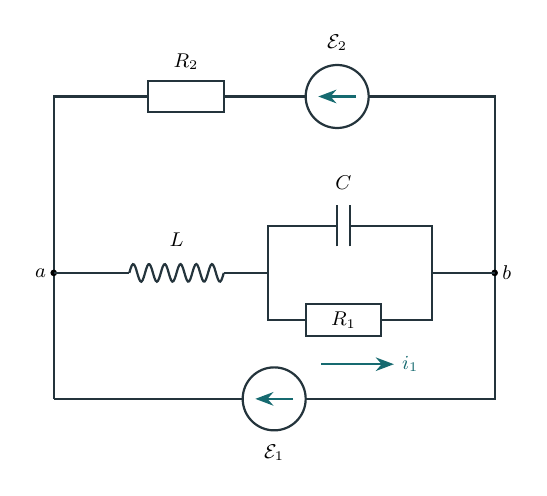
\begin{tikzpicture}[scale=.8,transform shape]

\draw[object] (0,-2)--(0,2.8)--(1.5,2.8);
\draw[object] (1.5,2.55) rectangle (2.7,3.05);
\draw[object] (2.7,2.8)--(4,2.8);
\draw[object] (4.5,2.8) circle (.5);
\draw[object] (5,2.8)--(7,2.8)--(7,-2)--(4,-2);
\draw[object] (3.5,-2) circle (.5);
\draw[object] (3,-2)--(0,-2);
\draw[motion] (3.8,-2)--(3.2,-2);
\draw[motion] (4.8,2.8)--(4.2,2.8);
\node[above] at (2.1,3.1) {$R_2$};
\node[above] at (4.5,3.4) {$\mathcal E_2$};
\node[below] at (3.5,-2.6) {$\mathcal E_1$};
\fill (0,0) circle (1.5pt) node[left] {$a$};
\fill (7,0) circle (1.5pt) node[right] {$b$};
\draw[object] (0,0)--(1.2,0);
\draw[object,domain=0:1.5,samples=80] plot ({1.2+\x},{.14*sin(1440*\x)});
\draw[object] (2.7,0)--(3.4,0)--(3.4,.75)--(4.5,.75);
\draw[object] (4.5,.42)--(4.5,1.08);\draw[object] (4.7,.42)--(4.7,1.08);
\draw[object] (4.7,.75)--(6,.75)--(6,-.75)--(5.2,-.75);
\draw[object] (4,-1) rectangle (5.2,-.5);
\draw[object] (4,-.75)--(3.4,-.75)--(3.4,0);
\draw[object] (6,0)--(7,0);
\node[above] at (1.95,.3) {$L$};
\node[above] at (4.6,1.2) {$C$};
\node at (4.6,-.75) {$R_1$};
\draw[motion] (4.25,-1.45)--(5.4,-1.45) node[right] {$i_1$};

\end{tikzpicture}
\figcaption{图电试3.3\quad 电源1直接固定母线电压，中支路为L串联电阻、电容的并联部分。}
\end{minipage}\end{center}

\par\vspace{5mm}\noindent{\small\color{muted}作答区}\par\vspace{3mm}\noindent\textcolor{rulegray}{\rule{\linewidth}{0.3pt}}\par\vspace{12mm}\noindent\textcolor{rulegray}{\rule{\linewidth}{0.3pt}}

\clearpage

\pdfbookmark[2]{第 4 题 三棱柱交流网络与最小补偿电容}{q4}

\section*{第 4 题\quad 三棱柱交流网络与最小补偿电容}\label{q:4}


三棱柱的上三角形为$ABC$、下三角形为$EDF$，对应连接棱为$AE,BD,CF$。九条棱各为相同的电阻$R$与电感$L$串联支路。给定角频率$\omega$下，$\omega L=\sqrt3R$。
\begin{enumerate}
\item 求$A,B$间等效复阻抗的模，答案用$R$表示。
\item 以$A,D$为输入输出端，在每一条支路中串联相同电容$C_1$，使整个网络功率因数为$1/\sqrt2$。求最小$C_1$。
\item 各支路不加电容，仅在网络$AD$外串一个电容$C_2$，使总串联组合功率因数为$1/\sqrt2$，求最小$C_2$。
\end{enumerate}
求最小值时须比较总无功为感性和容性两种可能。


\begin{center}\begin{minipage}{.98\linewidth}\centering
\begin{tikzpicture}[scale=.75,transform shape]

\coordinate (A) at (0,2.8);\coordinate (B) at (3.4,2.8);\coordinate (C) at (1.7,4.5);
\coordinate (E) at (0,0);\coordinate (D) at (3.4,0);\coordinate (F) at (1.7,1.7);
\draw[object] (A)--(B)--(C)--cycle;
\draw[object] (A)--(E)--(D)--(B);
\draw[guide] (E)--(F)--(D);\draw[guide] (C)--(F);
\foreach \p/\pos in {A/above left,B/right,C/above,D/below right,E/left,F/above left}
{\fill (\p) circle (1.5pt);\node[\pos] at (\p) {$\p$};}

\node[align=left] at (7,3) {九条棱各为串联$R,L$\\$z=R+j\sqrt3R$\\$|z|=2R$};
\node[align=left] at (7,.8) {端口一：$A,B$\\端口二：$A,D$};

\end{tikzpicture}
\figcaption{图电试3.4\quad 三棱柱的虚线棱也实际导电，端口选择决定等势结点。}
\end{minipage}\end{center}

\par\vspace{5mm}\noindent{\small\color{muted}作答区}\par\vspace{3mm}\noindent\textcolor{rulegray}{\rule{\linewidth}{0.3pt}}\par\vspace{12mm}\noindent\textcolor{rulegray}{\rule{\linewidth}{0.3pt}}

\clearpage

\pdfbookmark[2]{第 5 题 锯齿电源驱动的RC逐周期暂态}{q5}

\section*{第 5 题\quad 锯齿电源驱动的RC逐周期暂态}\label{q:5}


理想电容$C$、电阻$R$、开关$K$和理想电源串联，开始开路且电容不带电。$t=0$闭合开关。电源电动势周期为$T=RC$，在第$n$个完整周期内按
\[
\mathcal E(t)=\mathcal E_0\frac{t-nT}{T},
\qquad nT\le t<(n+1)T,\quad n=0,1,2,\ldots
\]
从零线性升至$\mathcal E_0$，到周期边界瞬间复位至零。
以$Q(t)$表示约定正极板上的带符号电荷，求$Q_N=Q(NT)$、$N=1,2,\ldots$及其$N\to\infty$的极限。给出任一周期内的电荷，并说明电源跳变时哪些量连续、连续时间解最终趋向何种状态。


\begin{center}\begin{minipage}{.98\linewidth}\centering
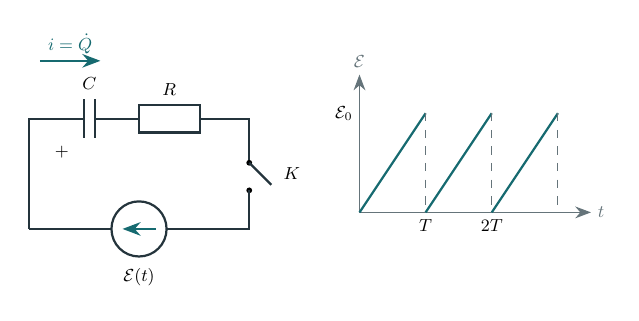
\begin{tikzpicture}[scale=.7,transform shape]

\draw[object] (0,0)--(0,2)--(1,2);
\draw[object] (1,1.65)--(1,2.35);\draw[object] (1.2,1.65)--(1.2,2.35);
\draw[object] (1.2,2)--(2,2);\draw[object] (2,1.75) rectangle (3.1,2.25);
\draw[object] (3.1,2)--(4,2)--(4,1.2);
\fill (4,1.2) circle (1.5pt);\fill (4,.7) circle (1.5pt);
\draw[object] (4,1.2)--(4.4,.8);\draw[object] (4,.7)--(4,0)--(2.5,0);
\draw[object] (2,0) circle (.5);\draw[object] (1.5,0)--(0,0);
\draw[motion] (2.3,0)--(1.7,0);
\node[above] at (1.1,2.4) {$C$};
\node[above] at (2.55,2.3) {$R$};
\node[right] at (4.5,1) {$K$};\node[below] at (2,-.6) {$\mathcal E(t)$};
\node at (.6,1.4) {$+$};\draw[motion] (.2,3.05)--(1.3,3.05) node[midway,above] {$i=\dot Q$};
\begin{scope}[xshift=6cm,yshift=.3cm]
\draw[axis] (0,0)--(4.2,0) node[right] {$t$};
\draw[axis] (0,0)--(0,2.5) node[above] {$\mathcal E$};
\foreach \n in {0,1,2}{\draw[traj] (\n*1.2,0)--({(\n+1)*1.2},1.8);
\draw[guide] ({(\n+1)*1.2},1.8)--({(\n+1)*1.2},0);}
\node[left] at (0,1.8) {$\mathcal E_0$};
\node[below] at (1.2,0) {$T$};\node[below] at (2.4,0) {$2T$};
\end{scope}

\end{tikzpicture}
\figcaption{图电试3.5\quad 电源在每个周期边界复位，正极板电荷由有限RC电流改变。}
\end{minipage}\end{center}

\par\vspace{5mm}\noindent{\small\color{muted}作答区}\par\vspace{3mm}\noindent\textcolor{rulegray}{\rule{\linewidth}{0.3pt}}\par\vspace{12mm}\noindent\textcolor{rulegray}{\rule{\linewidth}{0.3pt}}

\end{document}
